\section{Desenvolvimento Experimental}
\subsection{Materiais e Métodos}
Foram utilizados para a realização do experimento:
\begin{itemize}
	\item Tubo e/m;
	\item Duas bobinas de Helmholtz com 15 cm de raio;
	\item Régua espelhada;
	\item Duas fontes DC;
	\item Multímetros;
	\item Cabos de energia.
\end{itemize}

O experimento consiste em um tubo com gás rarefeito  ao qual é acoplado um filamento de metal. Liga-se o filamento a uma fonte em uma tensão menor que 6,0 $volts$, então ao passar uma corrente pelo fio este emitirá elétrons os quais serão defletidos em forma de feixe, que ionizarão o gás formando um rastro de luz. Em seguida, deve-se regular o foco do feixe através do botão a frente do equipamento. É submetido o tubo a um campo margnético uniforme por meio de uma bobina cuja corrente e voltagem podem ser controladas pelo painel frontal. O campo defletirá o fixe de elétrons em um círculo que poderá ser medido por uma régua ao fundo do tubo. Para se calcular a razão carga-massa é preciso variar a voltagem da bobina e consequentemente o raio ao qual o feixe é defletido. A variação é dada entre 150 e 300 $volts$ atingidas de 10 em 10 $volts$.

\subsection{Dados Obtidos Experimentalmente}
Após a realização do experimento duas vezes, foram obtidos diversos dados e utilizando os mesmos, foi gerado em programa o gráfico da Figura \ref{fig},contendo a diferença de potencial aplicada (DDP) com o respectivo raio do feixe de elétrons ($r$), e calculando o ajuste linear obteve-se a equação $V = 98079.57r^2 $

\begin{figure}[!ht]
	\centering
		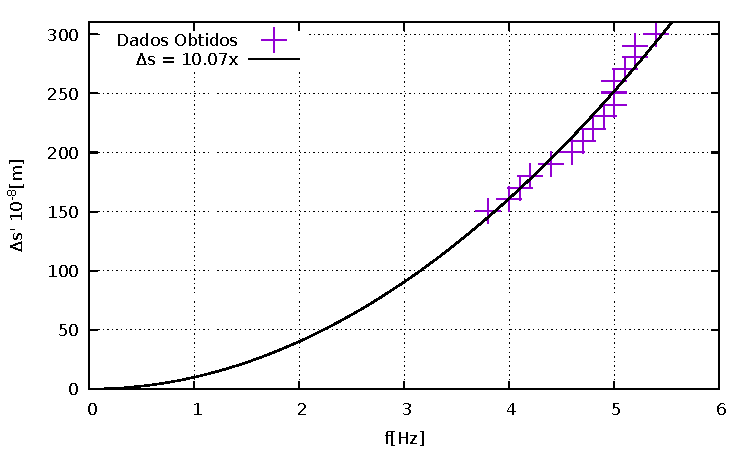
\includegraphics[scale= 1.0]{graf/e_m.pdf}
	\caption{Relação entre a diferença de potencial($DDP$) usado para acelerar os elétrons e o raio ($r$) formado pelos elétrons, com equação igual a $V = (98079.57\pm 1219.33)r^2$}
\label{fig}
\end{figure}

\subsection{Interpretação dos Resultados}

Sabendo-se que
\begin{equation}
	\frac{e}{m}=\frac{2V\left(\frac{5}{4}\right)^3a^2}{[N\mu _0 Ir]^2}
\end{equation}
é possível fazer
\begin{equation}
	V = \frac{[N \mu _0 I]^2\left(\frac{e}{m}\right)}{2(5/4)^3a^2}r^2
\end{equation}
onde fazendo
\begin{equation}
\begin{split}
	\lambda = \frac{[N \mu _0 I]^2\left(\frac{e}{m}\right)}{2(5/4)^3a^2}\\
	V = \lambda r^2
\label{eq1}
\end{split}
\end{equation}
sabendo que
\begin{equation}
	V = 98079,57r^2
\label{eq2}
\end{equation}
igualando \ref{eq1} e \ref{eq2} é obtido
\begin{equation*}
	\lambda = 98079,57
\end{equation*}
e portanto
\begin{equation}
	98079,57 =  \frac{[N \mu _0 I]^2\left(\frac{e}{m}\right)}{2(5/4)^3a^2}
\end{equation}
onde $N,\mu _0,I$ e $a$ são:
\begin{equation*}
	\begin{split}
		N=130\\
		\mu _0 =4\pi\times10^{-7}\\
		I=(1,24\pm0,01)A\\
		a=0,15cm
	\end{split}
\end{equation*}
substituindo os valores
\begin{equation}
	98079,57 =  \frac{[130*4\pi\times10^{-7}*1,24]^2\left(\frac{e}{m}\right)}{2(5/4)^30,15^2}
\end{equation}
e portanto
\begin{equation}
	\frac{e}{m}=\frac{98079,57*2*(5/4)^3*0,15^2}{[130*4\pi\times10^{-7}*124]^2}
\end{equation}
resolvendo
\begin{equation}
	\frac{e}{m}=(2,10\pm0,08)\times10^{11}Q/kg
\end{equation}
Comparando com o valor de 
\begin{equation}
	c=1,76\times10^{} Q/Kg
\end{equation}        
obtido na literatura \cite{PASCO}, resulta em um erro relativo ($Er$) de:
\begin{equation}
	Er=\left|\frac{1,76\times10^{11}-2,10\times10^{11}}{1,76\times10^{11}}\right|*100\%= 19,31\%
\end{equation}

Estes erros estão associados a obtenção dos dados, sendo
possível um erro de paralaxe durante a visualização dos dados na régua espelhada, o que acarreta uma variação do valor de $c$ predito na literatura. Porém, mesmo com todos os fatores associados, o erro  de
19,31\% é aceitável dentro da precisão necessária para a realização do experimento.

